\section{Desenvolvimento Teórico}
O feixe de luz que sai do laser é refletido em um ângulo $\theta$ com a reta normal do espelho rotatório ($MR$), como mostrado na $Figura 1$, em direção ao ponto $S$ do espelho fixo ($MF$). Ao passo que o espelho $MR$ rotaciona, sua reta normal irá variar em ângulo  $\Delta \theta$, resultando em um novo ângulo de incidência $\theta1$. O feixe incidirá então no ponto $S1$ do espelho $MF$.
\begin{figure}[!ht]
	\centering
	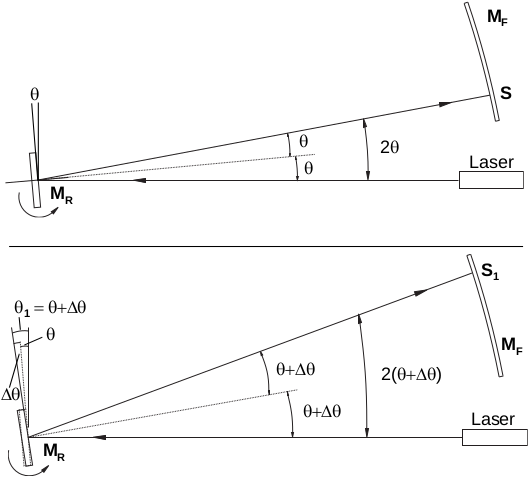
\includegraphics[scale=0.4]{2.png}
	\caption{Diagrama do caminho óptico percorrido pelo feixe e detalhe da diferença angular decorrente da rotação do espelho $MR$}
\end{figure} 
Sendo $D$ a distância entre os espelhos, a diferença de caminho entre os feixes é dada por:

\begin{equation}
	S1-S = D(2\theta1 - 2\theta)=D[2(\theta+\Delta\theta)-2\theta]= 2D\Delta		\theta
\end{equation}
Uma análise semelhante pode ser empregada na seguinte montagem:

\begin{figure}[!ht]
	\centering
	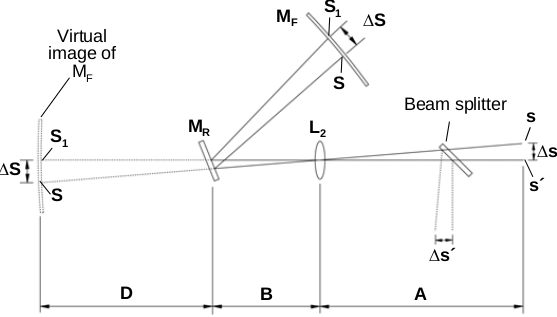
\includegraphics[scale=0.4]{3.png}
	\caption{Diagrama do caminho óptico semelhante ao arranjo experimental \cite{PASCO}}
\end{figure}
Onde o deslocamento do ponto imagem ($\Delta S'$) decorrente da rotação do espelho $MR$ é igual ao deslocamento $\Delta S$ da imagem virtual no espelho $MF$, a qual é determinada pela relação:

\begin{equation}
	\Delta S'= \Delta S=(-i/o)\Delta S
\end{equation}
Em que $i$ é a distância da imagem até a lente e $o$ a distância do objeto até a mesma ($L2$). Pela $Figura2$ obtem-se que:

\begin{equation}
	(-i/o)\Delta S=\frac{A}{D+B}\Delta S
\end{equation}
 
Substituindo o valor de $\Delta S$ obtido na eq. $1$:

\begin{equation}
	\Delta S'=\frac{2DA\Delta\theta}{D+B}
\end{equation}

Sabendo-se que o ângulo $\Delta\theta$ depende da velocidade de rotação ($\omega$) do espelho $MR$, do trajeto do feixe entre os espelhos ($2D$) e da velocidade $c$ da luz, resulta:

\begin{equation}
	\Delta\theta=\frac{2D\omega}{c}
\end{equation}

Com a igualdade da eq. $4$

\begin{equation}
	\Delta S'=\frac{4D^{2}A\omega}{c(D+B)}
\end{equation}

Isolando-se $c$:

\begin{equation}
	c=\frac{4D^{2}A\omega}{(D+B)\Delta S'}
\end{equation}

Variando então os parâmetros $\omega$ e, consequentemente, $\Delta S'$ e conhecendo os demais valores das constantes, é posível calcular a velocidade $c$ da luz.



